\chapter{GIẢI PHÁP THỰC HIỆN MÔ HÌNH DỰ ĐOÁN BỆNH XƠ PHỔI}
\section{Xây dựng và tiền xử lý tập dữ liệu}
\subsection{Tập dữ liệu}
Tập dữ liệu gồm $33202$ hình ảnh CT của $176$ bệnh nhân và các siêu dữ liệu về chỉ số FVC theo một số tuần được đo, giới tính, tuổi tác và tình trạng hút thuốc. $176$ bệnh nhân có độ tuổi từ 50 đến 90 trong đó phần đông các bệnh nhân có tuổi từ 60 đến 70. Về giới tính, đa phần là bệnh nhân nam. Về tình trạng hút thuốc là những người đã từng hút thuốc. Biểu đồ trong hình \ref{fig:data1} thể hiện dữ liệu về bệnh nhân.\par
\begin{figure}[ht!]
\centerline{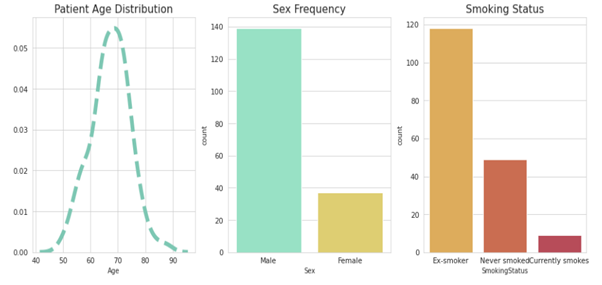
\includegraphics[scale=0.8]{images/data1.png}}
\caption{Biểu đồ thống kê thông tin của bệnh nhân trong tập dữ liệu}
\label{fig:data1}
\end{figure}

FVC (Forced Vital Capacity) hay dung tích sống gắng sức là lượng không khí thở ra nhanh và mạnh sau khi gắng sức hít thở sâu nhất có thể. FVC của các bệnh nhân sẽ được đo trong nhiều tuần trước, sau và ngay trong tuần chụp CT như hình \ref{fig:data2}. Tùy từng bệnh nhân mà thời gian đo có thể khác nhau, trải dài từ $5$ tuần trước khi hình CT được chụp $(-5)$ đến 133 tuần sau khi chụp CT $(133)$.\par
\begin{figure}[ht!]
\centerline{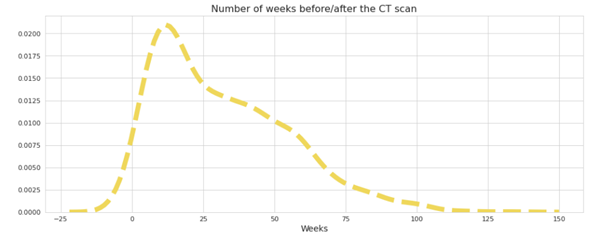
\includegraphics[scale=0.8]{images/data2.png}}
\caption{Thờì gian các ảnh CT được chụp}
\label{fig:data2}
\end{figure}
Về ảnh chụp CT các bệnh nhân, số lượng ảnh chụp CT các bệnh nhân cũng khác nhau. Ảnh chụp CT chụp liên tục phổi bệnh nhân trong một lần hít vào và khi quá trình hết một vòng tuần hoàn hô hấp hít vào như thế máy quét CT cũng dừng lại. Do đó, tùy vào tình trạng phổi mà bệnh nhân có thể hít sâu hay không khi đó số lượng ảnh chụp CT cũng khác nhau. Hình \ref{fig:data4} thể hiện ảnh chụp CT của một bệnh nhân. Hơn một nửa số lượng bệnh nhân có số lượng ảnh ít hơn 100 trong đó trung bình là 94 ảnh. Số lượng ảnh chụp CT của bệnh nhân được thể hiện ở hình \ref{fig:data3}.\par
\begin{figure}[ht!]
\centerline{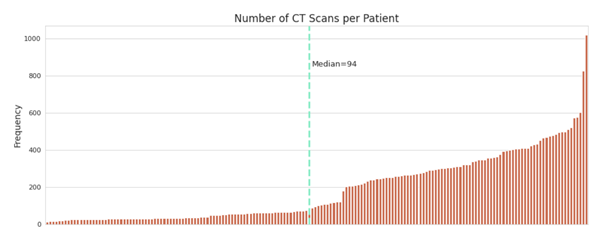
\includegraphics[scale=0.7]{images/data3.png}}
\caption{Số lượng ảnh chụp CT của từng bệnh nhân}
\label{fig:data3}
\end{figure}
\begin{figure}[ht!]
\centerline{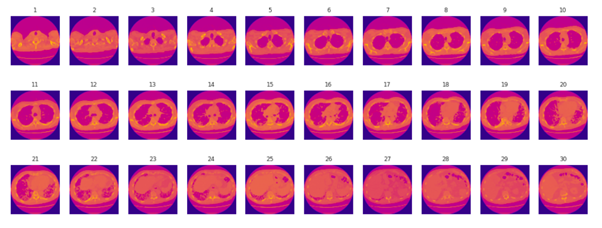
\includegraphics[scale=0.7]{images/data4.png}}
\caption{Ví dụ ảnh chụp CT trong một lần hít vào của 1 bệnh nhân}
\label{fig:data4}
\end{figure}
\subsection{Tiền xử lí ảnh}
Ảnh CT chụp thông tin về mật độ bức xạ của một thể hoặc các phần mô mềm khi tiếp xúc với tia X. Một lát cắt ngang của hình CT được tái cấu trúc sau khi các phép đo của tia X được thực hiện theo nhiều hướng khác nhau. Do vậy tùy thuộc vào các thành phần quang phổ do cài đặt thông số đo lường của các máy chụp CT mà mức xám của các pixel thể hiện phổi của bệnh nhân có thể khác nhau, hình ảnh phổi của bệnh nhân cũng to hay nhỏ tùy thuộc vào các thiết lập này.\par
\subsubsection{Biến đổi HU và thay đổi kích thước ảnh}
Đơn vị HU (Hounsfield Unit) ra đời để chuẩn hóa các mức xám của hình chụp CT. Và từ đơn vị HU này người ta cũng có thể xác định các thành phần có trong ảnh chụp CT như không khí, phổi, mỡ,... theo hình \ref{fig:data5}. Ảnh được chuyển qua đơn vị HU như hình \ref{fig:data6}\\
\begin{figure}[ht!]
\centerline{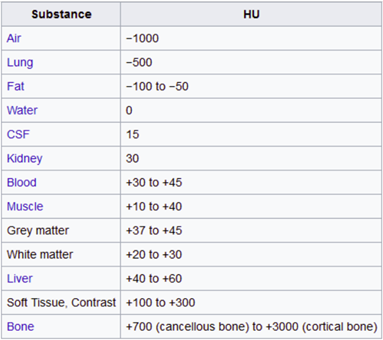
\includegraphics[scale=0.8]{images/data5.png}}
\caption{Đơn vị HU tương ứng với các thành phần trong ảnh chụp CT}
\label{fig:data5}
\end{figure}
Để đổi đơn vị HU, ta có thể áp dụng công thức sau: $U=m*SV + SI$.\\ 
Trong đó:\\
\tab m là giá trị bit đầu vào của ảnh chụp CT trước khi đổi sang HU.\\
\tab SV là giá trị Rescale Slope, một trong các tham số được lưu trong file dicom với tag là $(0028,1052)$.\\
\tab SI là giá trị Rescale Intercept, một trong các tham số được lưu trong file dicom với tag là $(0028,1053)$\\
\tab U là giá trị HU đầu ra.\par
\begin{figure}[ht!]
\centerline{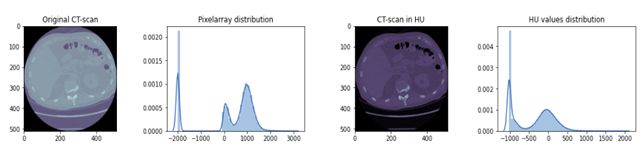
\includegraphics[scale=0.8]{images/data6.png}}
\caption{Ảnh chụp CT trước và sau khi chuyển đổi sang đơn vị HU}
\label{fig:data6}
\end{figure}
Ảnh sau khi được biến đổi HU để đồng nhất đơn vị cho các pixel, ta thực hiện thay đổi cắt và resize toàn bộ các ảnh về kích thước $512 x 512$. Bằng cách đổi toàn bộ các đơn vị ma trận về dạng int32 rồi thực hiện biến đổi sang hình ảnh nhờ thư viện Pillow. Từ hình ảnh sau khi được biến đổi, thực hiện cắt ảnh, đưa trở về dạng array nhờ thư viện Numpy và lưu lại ở dạng .npy.\\
\subsubsection{Phân đoạn ảnh chụp CT}
Sau khi đồng nhất các ảnh về kích thước $512 * 512$, dựa vào đơn vị HU ta có thể dễ dàng phân đoạn ảnh đối với vị trí phổi. Để phân đoạn phổi đầu tiên, thiết lập ngưỡng $-320$ đối với các pixel để xử lý sang ảnh nhị phân. Các pixel có giá trị thấp hơn $-320$ ta sẽ đưa về 0 còn những pixel lớn hơn $-320$ ta sẽ đưa về 1 (Hình \ref{fig:data7}). Khi này ta sẽ phân đoạn được 2 vùng:\\
\tab - Vùng có giá trị 0(trắng): Vùng không khí và phồi.\\
\tab - Vùng có giá trị 1(đen): Các vật thể khác.\par
\begin{figure}[ht!]
\centerline{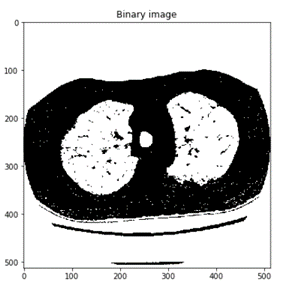
\includegraphics[scale=0.5]{images/data7.png}}
\caption{Ảnh chụp CT sau khi được phân ngưỡng -320 để tách làm 2 nhóm}
\label{fig:data7}
\end{figure}
Như vậy, ta chỉ cần phân đoạn được không khí và phổi với nhau thì sẽ thu được kết quả cuối cùng sau khi phân đoạn. Để thực hiện phân đoạn giữa phổi và không khí ta thực hiện phân đoạn bằng cách gán nhãn với các pixel có cùng giá trị ở cạnh nhau. Những pixel mang giá trị HU là không khí tập trung ở viền bức ảnh, do vậy với các pixel có cùng nhãn ta sẽ tăng thêm 1 để loại bỏ nó. Sau khi thực hiện, ta sẽ chỉ còn phần phổi và các đốm trắng nhiễu như hình \ref{fig:data8}:\par
\begin{figure}[ht!]
\centerline{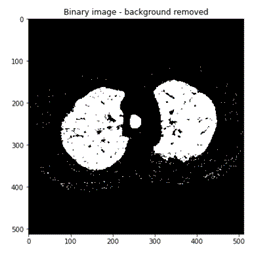
\includegraphics[scale=0.6]{images/data8.png}}
\caption{Ảnh chụp CT sau khi loại bỏ phần không khí}
\label{fig:data8}
\end{figure}
Kế đó, để loại bỏ nhiễu ta sẽ áp dụng hình thái đóng (closing morphology). Closing morphology thực hiện 2 phép toán giãn nở rồi xói màn. Với phép giãn nở, các bit có giá trị 1 sẽ được giãn nở với filter là một hình dĩa có bán kính là 2. Sau khi thực hiện phép giãn nở các chấm nhiễu sẽ biến mất và ta thực hiện phép xói màn với filter có cùng kích thước để đưa hình về ban đầu (Hình \ref{fig:data9}).\par
\begin{figure}[ht!]
\centerline{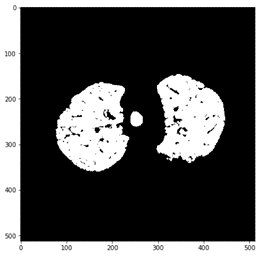
\includegraphics[scale=0.6]{images/data9.png}}
\caption{Ảnh chụp CT sau khi được phân đoạn}
\label{fig:data9}
\end{figure}
Kết quả cuối cùng sẽ trở thành mask để lọc các giá trị pixel nằm ở vị trí của phổi trong ảnh được lưu ở dạng .npy ở phần resize ảnh. Cuối cùng ta thu được ảnh đã được lọc vị trí của phổi và lưu nó ở dạng .png bằng mode = "gray" của thư viện matplolib (Hình \ref{fig:data10}).
\begin{figure}[ht!]
\centerline{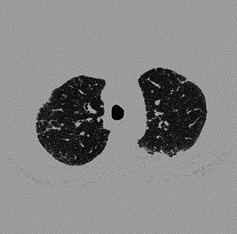
\includegraphics[scale=0.6]{images/data10.png}}
\caption{Ảnh chụp CT đã được lọc vị trí của phổi}
\label{fig:data10}
\end{figure}
\section{Xây dựng mô hình dự đoán FVC}
Để thực hiện dự đoán, mô hình được xây dựng gồm 2 mô hình con là Efficient Net và Quantile Regression. Dữ liệu hình ảnh chụp CT và các dữ liệu của bệnh nhân sẽ được đưa vào Efficient Net, lúc này Efficient Net có nhiệm vụ dự đoán hệ số góc của phương trình giữa FVC và tuần của bệnh nhân rồi từ đó suy ra FVC. Do phương trình đường thẳng giữa FVC và tuần là đường thẳng gần đúng mà không thể hiện được chính xác được mối quan hệ giữa FVC và tuần, khi đó các FVC đã dự đoán được ở mô hình Efficient Net (EN) sẽ tiếp tục được đưa và mô hình hồi quy Quantile Regression (QR) một lần nữa cùng với các dữ liệu của bệnh nhân để từ đó dự đoán FVC. FVC cuối cùng sẽ được tính theo công thức sau:\par
\begin{equation}
FVC= FVC(EN)*0.55 +FVC(QR)*0.45
\end{equation}
\subsection{Huấn luyện mô hình Efficient Net}
\subsubsection{Chuẩn bị dữ liệu}
Ở mô hình Efficient Net ta thực hiện dự đoán dựa trên các hình chụp CT. Tuy nhiên do tập dữ liệu quá lớn nên RAM của Google Colab không thể xử lý toàn bộ ảnh của bệnh nhân được. Trong tập dữ liệu ảnh chụp CT của các bệnh nhân thông thường sẽ gồm 3 giai đoạn: bắt đầu hít sâu, thực hiện hít sâu và bắt đầu thở ra. Do đó để giải quyết về vấn đề RAM của Google Colab, mỗi bệnh nhân nhóm chỉ chọn ra ngẫu nhiên 1 hình trong từng giai đoạn đó. Như vậy với dữ liệu đầu vào là ảnh chụp CT ta có 3 hình x 176 bệnh nhân. Vậy kích thước ngõ vào là $(528,64,64)$.\par
Các dữ liệu khác về độ tuổi, giới tính và tình trạng hút thuốc cũng ảnh hưởng đến FVC, vì vậy các dữ liệu cũng sẽ được mã hóa để đưa vào mô hình. Đối với độ tuổi, ta sẽ chuẩn hóa dữ liệu về quanh mức 1. Đối với giới tính, 0 sẽ là nam, 1 sẽ là nữ. Đối với tình trạng hút thuốc, “00” là chưa từng hút thuốc, “11” là đã từng hút thuốc, “01” là hiện đang hút thuốc.
Với từng bệnh nhân, từ các giá trị FVC và tuần, tìm ra đường thẳng xấp xỉ mối quan hệ giữa FVC và tuần rồi từ đó lưu lại hệ số góc của đường thẳng này (a) làm mục tiêu cho việc huấn luyện mô hình Efficient Net.\par
\begin{figure}[ht!]
\centerline{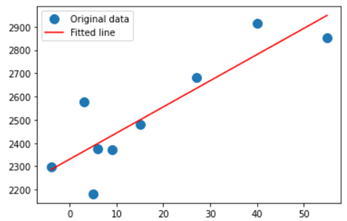
\includegraphics[scale=0.6]{images/train1.png}}
\caption{Phương trình đường thẳng (màu đỏ) quan hệ giữa tuần (trục hoành) và FVC(trục tung) và FVC chính xác theo từng tuần (chấm màu xanh) của bệnh nhân “ID00076637202199015035026”}
\label{fig:train1}
\end{figure}
\subsubsection{Mô hình huấn luyện Efficient Net}
Cài đặt thông số: \\
\tab - Epoch: 30\\
\tab - Batch size: 8\\
\tab - Learning rate: 0.03 \\
\tab - Số bước trong một Epoch: 32 (tập huấn luyện) và 16 (tập đánh giá)\\
\tab - Mô hình tối ưu theo dạng Adam Optimization.\par
Mô hình  được thư viện Keras cài đặt sẵn, như vậy chỉ cần xài mô hình đã được Keras cài sẵn để huấn luyện cho hình chụp CT. Ảnh chụp CT sau khi đi qua Efficient Net được lấy Pooling như sau:\par

\begin{center}
\begin{tabular} {|c|c|c|c|c|}
\hline
Lớp & Đầu vào & Kích thước & Đầu ra & Kích thước \\
 & & đầu vào & &đầu ra\\
\hline
Efficient Net & Ảnh chụp CT & $(64,64,1) $ & X1 & \\
\hline
GlobalPooling2D &	X1 & & X2 & $(1,1,1)$\\
\hline
Concatenate & [X2,dữ liệu] & $(1,1,1)*(4,1,1)$ & X3 & (5,1,1)\\
\hline
Drop out & X3 & (5,1,1) & X4 & (5,1,1)\\
\hline
Fully Connected & X4 & (5,1,1) & a & (1,1,1)\\
\hline
\end{tabular}
\label{tab:train1}
\end{center}
Sau khi quá trình huấn luyện kết thúc, ta sẽ có được file các hệ số của mô hình được lưu ở dạng file .h5.
\subsubsection{Dự đoán FVC từ mô hình Efficient Net}
Toàn bộ hình ảnh bệnh nhân trong tập kiểm tra sau khi tiền xử lý sẽ cùng với các thông số của bệnh nhân đi qua mô hình Efficient Net đã được huấn luyện để dự đoán hệ số góc của phương trình đường thẳng giữa FVC và tuần (a). Vì ở tập kiểm tra này ta đưa toàn bộ hình và với mỗi hình lại dự đoán ra được một a cho bệnh nhân. Vì vậy, với mỗi bệnh nhân được dự đoán rất nhiều a (do mỗi bệnh nhân lại có rất nhiều hình chụp CT)  xác suất a dự đoán có dạng xác phân phối Gauss, và a cuối cùng đại diện cho kết quả dự đoán của một bệnh nhân sẽ là giá trị ở đỉnh của xác suất Gauss này (tức là giá trị Q2 ở hình \ref{fig:train2}.\par
\begin{figure}[ht!]
\centerline{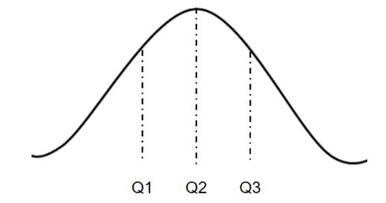
\includegraphics[scale=0.7]{images/train2.png}}
\caption{Phân phối Gauss}
\label{fig:train2}
\end{figure}
Từ a sau khi dự đoán, FVC của 1 tuần được đo để tìm ra giá trị b của phương trình đường thẳng $FVC = a*Tuần + b$. Từ phương trình đường thẳng vừa được xác lập tìm FVC từng tuần theo đường thẳng này. Khoảng sai lệch có thể tin tưởng (Confidence) được tính bằng công thức sau:
\begin{equation}
Confidence = Percent - A*|Week[test] - week|
\end{equation}
Trong đó :\\ 
\tab Percent là một trường tính toán xấp xỉ phần trăm độ giữa FVC của bệnh nhân với FVC của những người có tình trạng tương tự.\\
\tab A là hệ số góc của phương trình đường thẳng vừa tìm được.\\
\tab Week[test] là một số tuần được cho trong tập test.\\
\tab week là tuần cần dự đoán.

\subsection{Huấn luyện mô hình Quantile Regression}
Các FVC vừa tìm được ở mô hình Efficient Net là các FVC dựa vào phương trình đường thẳng mà tìm được do vậy các FVC ở đây vẫn không chính xác, cần xây dựng thêm mô hình hồi quy tuyến tính để dự đoán.
\subsubsection{Chuẩn bị dữ liệu}
Ở bước này, dữ liệu ở tập train được sử dụng để huấn luyện, dữ liệu tập test để đánh giá và tập sub để kiểm tra.Các dữ liệu được đưa vào mô hình gồm:
\tab - Male: “1” nếu bệnh nhân mang giới tính là nam\\
\tab - Female: “1” nếu bệnh nhân mang giới tính là nữ\\
\tab - Ex-smoker : “1” nếu bệnh nhân đã từng hút thuốc\\
\tab - Never smoked : “1” nếu bệnh nhân chưa từng hút thuốc\\
\tab - Currently smokes: “1” nếu bệnh nhân vẫn đang hút thuốc\\
\tab - Age: Chuẩn hóa tuổi bệnh nhân về trong khoảng [0:1]\\
\tab - Week: Chuẩn hóagiá trị FVC của các bệnh nhân về từ [0:1]\\
\tab - Base: Điều chỉnh lại tuần cần dự đoán với tuần đầu tiên cần xác định là tuần 0\par
Các thông số của mô hình với tối ưu Adam (Adam Optimizer)  được thiết lập như sau:	Learning rate: 0.1; $\beta_1:0.9$; $\beta_2: 0.999$; epoch: 600; batch size:8.\par
\subsubsection{Xây dựng mô hình}
Mô hình hồi quy tuyến tính Quantile Regression được mô tả như bảng sau:\par
\begin{center}
\begin{tabular} {|c|c|c|c|c|}
\hline
Lớp & Đầu vào & Kích thước & Đầu ra & Kích thước \\
 & & đầu vào & &đầu ra\\
\hline
Fully Connected 1 & Dữ liệu bệnh nhân & $(767,8) $ & d1 & $(767,100)$ \\
\hline
Fully Connected 2 & d1 & $(767,100)$ & d2 &$(767,100)$ \\
\hline
Fully Connected 3 & d2 &$(767,100)$ & p1 &$(767,3)$ \\
\hline
Fully Connected 4 & d2 &$(767,100)$ & p2 &$(767,3)$ \\
\hline
Lambda & [p1,p2] & [(767,3)(767,3)] & preds & (767,3)\\
\hline
\end{tabular}
\label{tab:train1}
\end{center}
Ở lớp cuối Lambda không thực hiện các tích chập mà được tính như sau: $$pred = p1+ cumsum(p2)$$
Trong đó:\\
\tab pred là ma trận dự đoán đầu ra ở lớp cuối\\
\tab p1 là ma trận đầu vào thứ nhất\\
\tab cumsum(p2) là tổng cộng dồn các giá trị của ma trận đầu vào thứ 2 qua 767 bệnh nhân\par
Ma trận đầu ra thực hiện dự đoán 3 giá trị là 3 giá trị FVC với mức lượng tử lần lượt là 0.2, 0.5, 0.8 tức là 3 giá trị Q1, Q2, Q3 theo hình \ref{fig:train2} . Trong đó mức lượng tử 0.5 là giá trị FVC dự đoán, FVC trong khoảng từ 0.2 đến 0.8 là mức sai số tin tưởng được (Confidence) của mô hình.
Hàm mất mát (Loss function) của mô hình được tính như sau:
$$L= 0.8* Mean( max(q*(y_{true} -y_{prediction}),(q-1)* (y_{true} - y_{prediction}))) + (1-0.8)* score$$
Trong đó:\\
\tab L là giá trị mất mát\\
\tab q là các ngưỡng lượng tử [0.2 0.5 0.8]\\
\tab $y_{true}$ là giá trị kết quả chính xác\\
\tab $y_{prediction}$ là giá trị kết quả do mô hình dự đoán\\
\tab score là hàm đánh giá dựạ trên kỹ thuật đánh giá Laplace Log Likehood.\par
Laplace Log Likelihood là phương pháp đánh giá được sử dụng trong y học để đánh giá độ chính xác của các mô hình. Mô hình được xây dựng để phản ánh cả độ sự chính xác và mức độ tin tưởng trên từng dự đoán. Mô hình cụ thể như sau:
$$\sigma = y_{prediction}[q=0.8] - y_{prediction}[q=0.2]$$
$$FVC_{prediction} = y_{prediction}[q=0.5]$$
$$\sigma_{clipped} = max(\sigma,70)$$
$$\Delta = min(\vert FVC_{true} - FVC_{prediction} \vert, 1000)$$
$$score = -\dfrac{\sqrt{2}\Delta}{\sigma_{clipped}} - ln(\sqrt{2}\sigma_clipped)$$
\par Để tránh việc sai số dự đoán quá lớn ảnh hưởng đến dự đoán, ngưỡng 1000 được thiết lập. Mức thấp nhất của khoảng sai số tin tưởng được được thiết lập ở ngưỡng 70.
\subsubsection{Dự đoán FVC của mô hình Quantile Regression và kết quả dự đoán FVC cuối cùng}
FVC cuối cùng của mô hình được dự đoán từ giá trị lượng tử q = 0.5 của mô hình. Trong khi đó, giá trị tin tưởng (Confidence) là hiệu của giá trị FVC với mới lượng tử q = 0.8 và giá trị FVC với mức lượng tử q = 0.2.
\begin{figure}[ht!]
\centerline{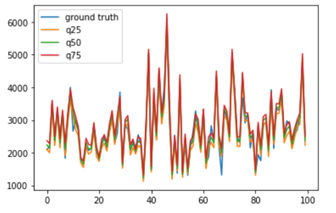
\includegraphics[scale=0.7]{images/train3.png}}
\caption{: Giá trị FVC với 3 mức lượng tử q = 0.2 (màu cam), q =0.5 (màu xanh lá), q = 0.75 (màu đỏ) và FVC chính xác (màu xanh) của tập đánh giá}
\label{fig:train3}
\end{figure} 